
\begin{multicols*}{2}

\section{Hunter}

\lettrine[lines=3, lhang=0.15, loversize=0.25, findent=.5em]{H}{unters} have undergone extensive training, ruthless mental and physical conditioning in preparation for facing all the sorts of beasts, demons, and aberrations.

\subsection*{Wanderer}

The hunter's nomadic culture allows them to adapt to the most inhospitable environments. For example, a hunter traveling through a marsh or a rain forest will quickly learn about edible and poisonous mushrooms, therefore gaining resistance to poison damage.



\begin{itemize}
    \item You have advantage on initiative rolls.
    \item You gain you proficiency with medium armor, and martial weapons.
    \item You gain resistance to either poison, cold or fire damage. Whenever you finish a long rest, you may change your damage resistance type.
    \item When you engage in two-weapon fighting, you can add your ability modifier to the damage of the second attack.    
\end{itemize}


\subsection*{Predator's Cunning}

At 3rd level, you learn maneuvers that are fueled by your cunning dice. Refer to the hunter's cunning action table for details.

\subsection*{Bird's Talons}

Starting at 5th level, you can attack twice, instead of once, whenever you take the Attack action on your turn.

If you don't have any cunning points at the start of a combat, you can burn a spell slot and have one cunning point per spell slot level instead.

\subsection*{Claw and Fang}

At 9th level, you become a legendary hunter. You gain several benefits, depending on your fighting style:

\begin{itemize}
    \item \textbf{Sword \& Shield:} When a creature hits you with an attack, you gain a +4 bonus to AC against all subsequent attacks made by that creature for the rest of the turn.
    \item \textbf{Two-weapon fighting:} You score critical-hits on 19-20
    \item \textbf{Bowmanship:} Once per turn, you can reduce the movement speed of a creature hit by your arrows by 10 feet.
\end{itemize}

\begin{Figure}
\centering
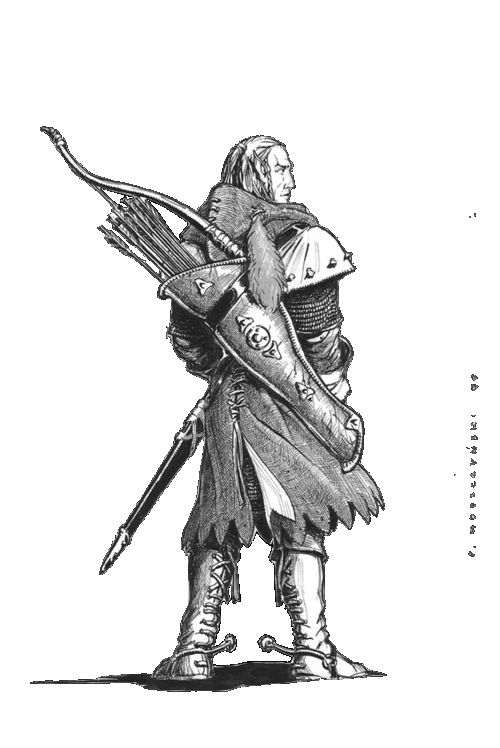
\includegraphics[width=\textwidth]{img/longbow.png}
\end{Figure}
    
\end{multicols*}


\clearpage

\begin{table}[ht!]
\begin{small}
\rowcolors{2}{}{commentgreen}
\begin{center}
\begin{tabular}{ll}
\multicolumn{2}{l}{\parbox[l][0.6cm][c]{15cm}{\textbf{Hunter Cunning Actions}}} 
\\
\hline 
\textbf{Name} & \parbox[l][0.6cm][c]{15cm}{\textbf{Description}}
\\ 
Rain of Arrows & \parbox[l][2.1cm][c]{15cm}{
As a reaction, you can spend one cunning point to make an attack of opportunity against any creature entering a space 15 feet away from you provided that you are holding a \hl{ranged} weapon.  If you hit, you add the cunning die to the attack's damage roll. Additionally, any feats or benefits applied only to melee weapons apply to your attack.
}
\\ 
Giant Killer & \parbox[l][2cm][c]{15cm}{
When a Large or larger creature within 5 feet of you hits or misses you with an attack, you can use a cunning point to spend your reaction to attack that creature immediately after its attack, provided that you can see the creature.  If you hit, you add the cunning die to the attack's damage roll.
}
\\ 
Augmenting Concoction & \parbox[l][2cm][c]{15cm}{
You can use your bonus action to 
spend one cunning point
 and drink a special potion 
that is toxic to any creature other than you. On you, 
the concotion makes you stronger. Until the end of your next turn, add your cunning die as extra damage to your attack rolls.
}
\\
Mercury Weapon & \parbox[l][2.1cm][c]{15cm}{
You can use your bonus action to 
spend one cunning point and dilute a mercury like chemical element over a pair of \hl{melee} weapons or \hl{20 missiles}. For the next 10 minutes, your weapons count as magical for the purpose of overcoming magical resistance
and receive a +1 bonus to attack and damage rolls.
}
\\
Herbal Vigor & \parbox[l][1.8cm][c]{15cm}{
You can use your bonus action to 
spend one cunning point and chew a special set or herbs to strengthen your immune system. For 1 hour, 
you gain resistance to poison damage and you gain temporary hit points equals to your cunning die.
}
\\
\hline
\end{tabular}
\end{center}
\end{small}
\end{table} 


\begin{multicols*}{2}
\begin{Figure}
\centering
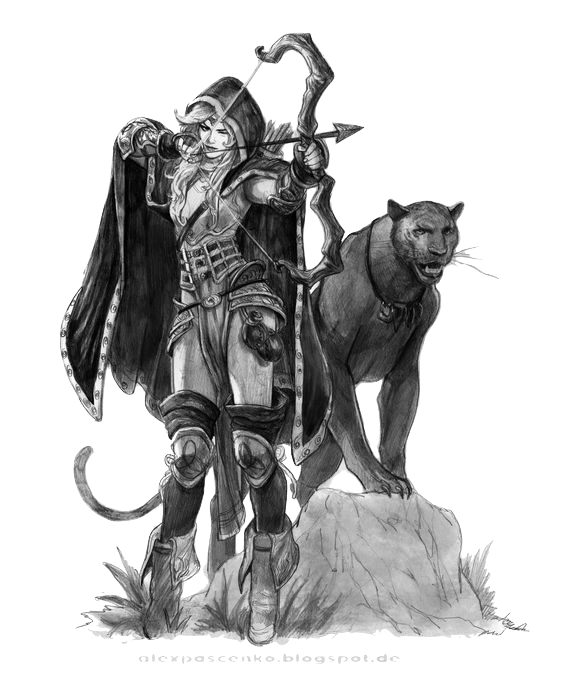
\includegraphics[width=\textwidth]{img/hunter-panther.png}
\end{Figure}
    
\end{multicols*}    